%% -*- mode: LaTeX; TeX-master: "../Summer14.tex" -*-
\section{Upper limits on \mtau LFV branching fractions}
\label{sec:tau:lfv}
We report in Table~\ref{tab:tau:lfv-upper-limits} and
Figure~\ref{fig:tau:lfv-limits-plot} the up-to-date upper
limits on the \mtau LFV branching fractions in order to track and
summarize the experimental results in this area, which are sensitive
to physics beyond the Standard Model.
\begin{center}
\begin{longtable}{lcl@{}rll}
\caption{Experimental upper limits on lepton flavor violating \mtau
  decays. The modes are grouped according to the particle content of their final
  states. Modes with lepton number violation are labeled with ``(L)'',
  modes with baryon number violation are labeled with ``(BNV)''.
  \label{tab:tau:lfv-upper-limits}}%
\\
\toprule
\multicolumn{1}{l}{\bfseries Decay mode} &
\multicolumn{1}{l}{\bfseries Category} &
\multicolumn{2}{c}{\bfseries \begin{tabular}{@{}c@{}}90\% CL\\Limit\end{tabular}} &
\multicolumn{1}{l}{\bfseries Exp.} &
\multicolumn{1}{l}{\bfseries Ref.} \\
\midrule
\endfirsthead
\multicolumn{6}{c}{{\bfseries \tablename\ \thetable{} -- continued from previous page}} \\ \midrule
\multicolumn{1}{l}{\bfseries Decay mode} &
\multicolumn{1}{l}{\bfseries Category} &
\multicolumn{2}{c}{\bfseries \begin{tabular}{@{}c@{}}90\% CL\\Limit\end{tabular}} &
\multicolumn{1}{l}{\bfseries Exp.} &
\multicolumn{1}{l}{\bfseries Ref.} \\
\midrule
\endhead
%
%  l\gamma
%   
\begin{ensuredisplaymath}
\Gamma_{156} =  {e^- \gamma} 
\end{ensuredisplaymath}
 &\(l\gamma\) & \( <\; \) & \(12.0 \cdot 10^{-8}\)         & Belle &  \cite{Hayasaka:2007vc} \\
 &            & \( <\; \) & \(3.3 \cdot 10^{-8}\)         & \babar &  \cite{Aubert:2009ag}   \\ 
%\midrule
\begin{ensuredisplaymath}
\Gamma_{157} =  {\mu^- \gamma} 
\end{ensuredisplaymath}
 &            & \( <\; \) & \(4.5 \cdot 10^{-8}\)         & Belle &  \cite{Hayasaka:2007vc} \\
 &            & \( <\; \) & \(4.4 \cdot 10^{-8}\)         & \babar &  \cite{Aubert:2009ag}   \\ 
\midrule
%
%  lP0
% 
\begin{ensuredisplaymath}
\Gamma_{158} =  {e^- \pi^0} 
\end{ensuredisplaymath}
 &\(lP^0 \)   & \( <\; \) & \(2.2 \cdot 10^{-8}\)         & Belle & \cite{Hayasaka:2011zz} \\
 &            & \( <\; \) & \(13.0 \cdot 10^{-8}\)         & \babar & \cite{Aubert:2006cz} \\ 
%\midrule
\begin{ensuredisplaymath}
\Gamma_{159} =  {\mu^- \pi^0} 
\end{ensuredisplaymath}
 &            & \( <\; \) & \(2.7 \cdot 10^{-8}\)         & Belle &  \cite{Hayasaka:2011zz}  \\
 &            & \( <\; \) & \(11.0 \cdot 10^{-8}\)         & \babar &  \cite{Aubert:2006cz} \\ 
%\midrule
\begin{ensuredisplaymath}
\Gamma_{162} =  {e^- \eta} 
\end{ensuredisplaymath}
 &            & \( <\; \) & \(4.4 \cdot 10^{-8}\)         & Belle &  \cite{Hayasaka:2011zz}  \\
 &            & \( <\; \) & \(16.0 \cdot 10^{-8}\)         & \babar &  \cite{Aubert:2006cz} \\ 
%\midrule
\begin{ensuredisplaymath}
\Gamma_{163} =  {\mu^- \eta} 
\end{ensuredisplaymath}
 &            & \( <\; \) & \(2.3 \cdot 10^{-8}\)         & Belle &   \cite{Hayasaka:2011zz} \\
 &            & \( <\; \) & \(15.0 \cdot 10^{-8}\)         & \babar &   \cite{Aubert:2006cz} \\ 
%\midrule
\begin{ensuredisplaymath}
\Gamma_{172} =  {e^- \eta'(958)} 
\end{ensuredisplaymath}
 &            & \( <\; \) & \(3.6 \cdot 10^{-8}\)         & Belle &   \cite{Hayasaka:2011zz}  \\
 &            & \( <\; \) & \(24.0 \cdot 10^{-8}\)         & \babar &   \cite{Aubert:2006cz} \\ 
%\midrule
\begin{ensuredisplaymath}
\Gamma_{173} =  {\mu^- \eta'(958)} 
\end{ensuredisplaymath}
 &            & \( <\; \) & \(3.8 \cdot 10^{-8}\)         & Belle &   \cite{Hayasaka:2011zz}  \\
 &            & \( <\; \) & \(14.0 \cdot 10^{-8}\)         & \babar &   \cite{Aubert:2006cz} \\ 
%\midrule
\begin{ensuredisplaymath}
\Gamma_{160} =  {e^- K^0_S} 
\end{ensuredisplaymath}
 &            & \( <\; \) & \(2.6 \cdot 10^{-8}\)         & Belle &  \cite{Miyazaki:2010qb} \\
 &            & \( <\; \) & \(3.3 \cdot 10^{-8}\)         & \babar &  \cite{Aubert:2009ys}   \\ 
%\midrule
\begin{ensuredisplaymath}
\Gamma_{161} =  {\mu^- K^0_S} 
\end{ensuredisplaymath}
 &            & \( <\; \) & \(2.3 \cdot 10^{-8}\)         & Belle &   \cite{Miyazaki:2010qb} \\
 &            & \( <\; \) & \(4.0 \cdot 10^{-8}\)         & \babar &   \cite{Aubert:2009ys}   \\ 
\midrule
%
%  l S^0
%
\begin{ensuredisplaymath}
\Gamma_{174} =  {e^- f_0(980)} 
\end{ensuredisplaymath}
 &  \(l S^0\) & \( <\; \) & \(3.2 \cdot 10^{-8}\)         & Belle & \cite{Miyazaki:2008mw}\\
%&            & \( <\; \) & \(1.0 \cdot 10^{-8}\)         & \babar &                       \\ 
%\midrule
\begin{ensuredisplaymath}
\Gamma_{175} =  {\mu^- f_0(980)} 
\end{ensuredisplaymath}
 &            & \( <\; \) & \(3.4 \cdot 10^{-8}\)         & Belle & \cite{Miyazaki:2008mw}\\  
%&            & \( <\; \) & \(1.0 \cdot 10^{-8}\)         & \babar &                       \\ 
\midrule
%
% l V0
%
\begin{ensuredisplaymath}
\Gamma_{164} =  {e^- \rho^0} 
\end{ensuredisplaymath}
 &  \(l V^0\) & \( <\; \) & \(1.8 \cdot 10^{-8}\)         & Belle &  \cite{Miyazaki:2011xe}\\
 &            & \( <\; \) & \(4.6 \cdot 10^{-8}\)         & \babar &  \cite{Aubert:2009ap}  \\ 
%\midrule
\begin{ensuredisplaymath}
\Gamma_{165} =  {\mu^- \rho^0} 
\end{ensuredisplaymath}
 &            & \( <\; \) & \(1.2 \cdot 10^{-8}\)         & Belle &  \cite{Miyazaki:2011xe}\\
 &            & \( <\; \) & \(2.6 \cdot 10^{-8}\)         & \babar &  \cite{Aubert:2009ap}  \\ 
%\midrule
\begin{ensuredisplaymath}
\Gamma_{168} =  {e^- K^*(892)^0} 
\end{ensuredisplaymath}
 &            & \( <\; \) & \(3.2 \cdot 10^{-8}\)         & Belle &  \cite{Miyazaki:2011xe} \\
 &            & \( <\; \) & \(5.9 \cdot 10^{-8}\)         & \babar &  \cite{Aubert:2009ap}   \\ 
%\midrule
\begin{ensuredisplaymath}
\Gamma_{169} =  {\mu^- K^*(892)^0} 
\end{ensuredisplaymath}
 &            & \( <\; \) & \(7.2 \cdot 10^{-8}\)         & Belle &   \cite{Miyazaki:2011xe} \\
 &            & \( <\; \) & \(17.0 \cdot 10^{-8}\)         & \babar &   \cite{Aubert:2009ap}   \\ 
%\midrule
\begin{ensuredisplaymath}
\Gamma_{170} =  {e^- \bar{K}^*(892)^0} 
\end{ensuredisplaymath}
 &            & \( <\; \) & \(3.4 \cdot 10^{-8}\)         & Belle &   \cite{Miyazaki:2011xe} \\
 &            & \( <\; \) & \(4.6 \cdot 10^{-8}\)         & \babar &   \cite{Aubert:2009ap}   \\ 
%\midrule
\begin{ensuredisplaymath}
\Gamma_{171} =  {\mu^- \bar{K}^*(892)^0} 
\end{ensuredisplaymath}
 &            & \( <\; \) & \(7.0 \cdot 10^{-8}\)         & Belle &  \cite{Miyazaki:2011xe} \\
 &            & \( <\; \) & \(7.3 \cdot 10^{-8}\)         & \babar &  \cite{Aubert:2009ap}   \\ 
%\midrule

\begin{ensuredisplaymath}
\Gamma_{176} =  {e^- \phi} 
\end{ensuredisplaymath}
 &            & \( <\; \) & \(3.1 \cdot 10^{-8}\)         & Belle &   \cite{Miyazaki:2011xe} \\
 &            & \( <\; \) & \(3.1 \cdot 10^{-8}\)         & \babar &   \cite{Aubert:2009ap}   \\ 
%\midrule
\begin{ensuredisplaymath}
\Gamma_{177} =  {\mu^- \phi} 
\end{ensuredisplaymath}
 &            & \( <\; \) & \(8.4 \cdot 10^{-8}\)         & Belle &   \cite{Miyazaki:2011xe} \\
 &            & \( <\; \) & \(19.0 \cdot 10^{-8}\)         & \babar &   \cite{Aubert:2009ap}   \\ 
%\midrule
\begin{ensuredisplaymath}
\Gamma_{166} =  {e^- \omega} 
\end{ensuredisplaymath}
 &            & \( <\; \) & \(4.8 \cdot 10^{-8}\)         & Belle &  \cite{Miyazaki:2011xe} \\
 &            & \( <\; \) & \(11.0 \cdot 10^{-8}\)         & \babar &  \cite{Aubert:2007kx}   \\ 
%\midrule
\begin{ensuredisplaymath}
\Gamma_{167} =  {\mu^- \omega} 
\end{ensuredisplaymath}
 &            & \( <\; \) & \(4.7 \cdot 10^{-8}\)         & Belle &  \cite{Miyazaki:2011xe} \\
 &            & \( <\; \) & \(10.0 \cdot 10^{-8}\)         & \babar &  \cite{Aubert:2007kx}   \\ 
\midrule
%
% lll
%
\begin{ensuredisplaymath}
\Gamma_{178} =  {e^- e^+ e^-} 
\end{ensuredisplaymath}
 &  \(lll\)   & \( <\; \) & \(2.7 \cdot 10^{-8}\)         & Belle & \cite{Hayasaka:2010np} \\
 &            & \( <\; \) & \(2.9 \cdot 10^{-8}\)         & \babar & \cite{Lees:2010ez}     \\ 
%\midrule
\begin{ensuredisplaymath}
\Gamma_{181} =  {\mu^- e^+ e^-} 
\end{ensuredisplaymath}
 &            & \( <\; \) & \(1.8 \cdot 10^{-8}\)         & Belle & \cite{Hayasaka:2010np} \\
 &            & \( <\; \) & \(2.2 \cdot 10^{-8}\)         & \babar & \cite{Lees:2010ez}     \\ 
%\midrule
\begin{ensuredisplaymath}
\Gamma_{179} =  {e^- \mu^+ \mu^-} 
\end{ensuredisplaymath}
 &            & \( <\; \) & \(2.7 \cdot 10^{-8}\)         & Belle & \cite{Hayasaka:2010np} \\
 &            & \( <\; \) & \(3.2 \cdot 10^{-8}\)         & \babar & \cite{Lees:2010ez}     \\ 
%\midrule
\begin{ensuredisplaymath}
\Gamma_{183} =  {\mu^- \mu^+ \mu^-} 
\end{ensuredisplaymath}
 &            & \( <\; \) & \(2.1 \cdot 10^{-8}\)         & Belle & \cite{Hayasaka:2010np} \\
 &            & \( <\; \) & \(3.3 \cdot 10^{-8}\)         & \babar &
  \cite{Lees:2010ez}     \\ 
 &            & \( <\; \) & \(4.6 \cdot 10^{-8}\)         & \lhcb &
  \cite{Aaij:2014azz}     \\ 

%\midrule
\begin{ensuredisplaymath}
\Gamma_{182} =  {e^- \mu^+ e^-} 
\end{ensuredisplaymath}
 &            & \( <\; \) & \(1.5 \cdot 10^{-8}\)         & Belle & \cite{Hayasaka:2010np} \\
 &            & \( <\; \) & \(1.8 \cdot 10^{-8}\)         & \babar & \cite{Lees:2010ez}     \\ 
%\midrule
\begin{ensuredisplaymath}
\Gamma_{180} =  {\mu^- e^+ \mu^-} 
\end{ensuredisplaymath}
 &            & \( <\; \) & \(1.7 \cdot 10^{-8}\)         & Belle & \cite{Hayasaka:2010np} \\
 &            & \( <\; \) & \(2.6 \cdot 10^{-8}\)         & \babar & \cite{Lees:2010ez}     \\ 
\midrule
%
% l h h
%
\begin{ensuredisplaymath}
\Gamma_{184} =  {e^- \pi^+ \pi^-} 
\end{ensuredisplaymath}
 &    \(lhh\) & \( <\; \) & \(2.3 \cdot 10^{-8}\)         & Belle &  \cite{Miyazaki:2012mx}\\
 &            & \( <\; \) & \(12.0 \cdot 10^{-8}\)         & \babar &  \cite{Aubert:2005tp}  \\ 
%\midrule
\begin{ensuredisplaymath}
\Gamma_{186} =  {\mu^- \pi^+  \pi^-} 
\end{ensuredisplaymath}
 &            & \( <\; \) & \(2.1 \cdot 10^{-8}\)         & Belle &  \cite{Miyazaki:2012mx} \\
 &            & \( <\; \) & \(29.0 \cdot 10^{-8}\)         & \babar &  \cite{Aubert:2005tp}   \\ 
%\midrule
\begin{ensuredisplaymath}
\Gamma_{188} =  {e^- \pi^+ K^-} 
\end{ensuredisplaymath}
 &            & \( <\; \) & \(3.7 \cdot 10^{-8}\)         & Belle &  \cite{Miyazaki:2012mx} \\
 &            & \( <\; \) & \(32.0 \cdot 10^{-8}\)         & \babar &  \cite{Aubert:2005tp}   \\ 
%\midrule
\begin{ensuredisplaymath}
\Gamma_{194} =  {\mu^- \pi^+  K^-} 
\end{ensuredisplaymath}
 &            & \( <\; \) & \(8.6 \cdot 10^{-8}\)         & Belle &   \cite{Miyazaki:2012mx} \\
 &            & \( <\; \) & \(26.0 \cdot 10^{-8}\)         & \babar &   \cite{Aubert:2005tp}   \\ 
%\midrule
\begin{ensuredisplaymath}
\Gamma_{189} =  {e^- K^+ \pi^-} 
\end{ensuredisplaymath}
 &            & \( <\; \) & \(3.1 \cdot 10^{-8}\)         & Belle &   \cite{Miyazaki:2012mx} \\
 &            & \( <\; \) & \(17.0 \cdot 10^{-8}\)         & \babar &   \cite{Aubert:2005tp}   \\ 
%\midrule
\begin{ensuredisplaymath}
\Gamma_{195} =  {\mu^- K^+  \pi^-} 
\end{ensuredisplaymath}
 &            & \( <\; \) & \(4.5 \cdot 10^{-8}\)         & Belle &   \cite{Miyazaki:2012mx} \\
 &            & \( <\; \) & \(32.0 \cdot 10^{-8}\)         & \babar &   \cite{Aubert:2005tp}   \\ 
%\midrule

\begin{ensuredisplaymath}
\Gamma_{192} =  {e^- K^+ K^-} 
\end{ensuredisplaymath}
 &            & \( <\; \) & \(3.4 \cdot 10^{-8}\)         & Belle &   \cite{Miyazaki:2012mx} \\
 &            & \( <\; \) & \(14.0 \cdot 10^{-8}\)         & \babar &   \cite{Aubert:2005tp}   \\ 
%\midrule
\begin{ensuredisplaymath}
\Gamma_{198} =  {\mu^- K^+  K^-} 
\end{ensuredisplaymath}
 &            & \( <\; \) & \(4.4 \cdot 10^{-8}\)         & Belle &   \cite{Miyazaki:2012mx} \\
 &            & \( <\; \) & \(25.0 \cdot 10^{-8}\)         & \babar &   \cite{Aubert:2005tp}   \\ 
%\midrule
\begin{ensuredisplaymath}
\Gamma_{191} =  {e^- K^0_S K^0_S} 
\end{ensuredisplaymath}
 &            & \( <\; \) & \(7.1 \cdot 10^{-8}\)         & Belle &  \cite{Miyazaki:2010qb}  \\
%&            & \( <\; \) & \(1.0 \cdot 10^{-8}\)         & \babar &                       \\ 
%\midrule
\begin{ensuredisplaymath}
\Gamma_{197} =  {\mu^- K^0_S  K^0_S} 
\end{ensuredisplaymath}
 &            & \( <\; \) & \(8.0 \cdot 10^{-8}\)         & Belle &   \cite{Miyazaki:2010qb} \\
%&            & \( <\; \) & \(1.0 \cdot 10^{-8}\)         & \babar &                       \\ 
%\midrule
%
% lff, Lepton number violating modes.
%
\begin{ensuredisplaymath}
\Gamma_{185} =  {e^+ \pi^- \pi^- } 
\end{ensuredisplaymath}
 & (L)           & \( <\; \) & \(2.0 \cdot 10^{-8}\)         & Belle & \cite{Miyazaki:2012mx} \\
 & (L)           & \( <\; \) & \(27.0 \cdot 10^{-8}\)         & \babar & \cite{Aubert:2005tp}   \\ 
%\midrule
\begin{ensuredisplaymath}
\Gamma_{187} =  {\mu^+ \pi^- \pi^-} 
\end{ensuredisplaymath}
 & (L)        & \( <\; \) & \(3.9 \cdot 10^{-8}\)         & Belle &   \cite{Miyazaki:2012mx} \\
 & (L)        & \( <\; \) & \(7.0 \cdot 10^{-8}\)         & \babar &   \cite{Aubert:2005tp}   \\ 
%\midrule
\begin{ensuredisplaymath}
\Gamma_{190} =  {e^+ \pi^- K^- } 
\end{ensuredisplaymath}
 & (L)        & \( <\; \) & \(3.2 \cdot 10^{-8}\)         & Belle &   \cite{Miyazaki:2012mx} \\
 & (L)        & \( <\; \) & \(18.0\cdot 10^{-8}\)         & \babar &   \cite{Aubert:2005tp}   \\ 
%\midrule
\begin{ensuredisplaymath}
\Gamma_{196} =  {\mu^+ \pi^- K^-} 
\end{ensuredisplaymath}
 & (L)        & \( <\; \) & \(4.8 \cdot 10^{-8}\)         & Belle &   \cite{Miyazaki:2012mx} \\
 & (L)        & \( <\; \) & \(22.0 \cdot 10^{-8}\)         & \babar &   \cite{Aubert:2005tp}   \\ 
%\midrule
\begin{ensuredisplaymath}
\Gamma_{193} =  {e^+ K^- K^- } 
\end{ensuredisplaymath}
 &  (L)       & \( <\; \) & \(3.3 \cdot 10^{-8}\)         & Belle &   \cite{Miyazaki:2012mx} \\
 &  (L)       & \( <\; \) & \(15.0 \cdot 10^{-8}\)         & \babar &   \cite{Aubert:2005tp}   \\ 
%\midrule
\begin{ensuredisplaymath}
\Gamma_{199} =  {\mu^+ K^- K^-} 
\end{ensuredisplaymath}
 &  (L)       & \( <\; \) & \(4.7 \cdot 10^{-8}\)         & Belle &   \cite{Miyazaki:2012mx} \\
 &  (L)       & \( <\; \) & \(48.0 \cdot 10^{-8}\)         & \babar &   \cite{Aubert:2005tp}   \\ 
\midrule
%
% Lambda h
%
\begin{ensuredisplaymath}
\Gamma_{211} =  { \pi^- \Lambda } 
\end{ensuredisplaymath}
 & BNV & \( <\; \) & \(3.0 \cdot 10^{-8}\)         & Belle & \cite{Hayasaka:2012pj}  \\
 &               & \( <\; \) & \(5.8 \cdot 10^{-8}\)         & \babar &  \cite{Lafferty:2007zz}  \\ 
%\midrule
\begin{ensuredisplaymath}
\Gamma_{212} =  { \pi^- \bar{\Lambda}} 
\end{ensuredisplaymath}
 &            & \( <\; \) & \(2.8 \cdot 10^{-8}\)         & Belle & \cite{Hayasaka:2012pj}  \\
 &            & \( <\; \) & \(5.9 \cdot 10^{-8}\)         & \babar &  \cite{Lafferty:2007zz}  \\ 
%\midrule
\begin{ensuredisplaymath}
\Gamma_{213} =  { K^- \Lambda } 
\end{ensuredisplaymath}
 &            & \( <\; \) & \(4.2 \cdot 10^{-8}\)         & Belle &  \cite{Hayasaka:2012pj} \\
 &            & \( <\; \) & \(15.\cdot 10^{-8}\)         & \babar &  \cite{Lafferty:2007zz} \\ 
%\midrule
\begin{ensuredisplaymath}
\Gamma_{214} =  { K^- \bar{\Lambda}} 
\end{ensuredisplaymath}
 &            & \( <\; \) & \(3.1 \cdot 10^{-8}\)         & Belle & \cite{Hayasaka:2012pj}  \\
 &            & \( <\; \) & \(7.2 \cdot 10^{-8}\)         & \babar & \cite{Lafferty:2007zz}  \\ 
 \begin{ensuredisplaymath}
\Gamma_{215} =  { \proton \mu^- \mu^-} 
\end{ensuredisplaymath}
&            & \( <\; \) & \(44.0 \cdot 10^{-8}\)         & \lhcb & \cite{Aaij:2013fia}  \\
 \begin{ensuredisplaymath}
\Gamma_{216} =  { \bar{\proton} \mu^+ \mu^-} 
\end{ensuredisplaymath}
&            & \( <\; \) & \(33.0 \cdot 10^{-8}\)         & \lhcb & \cite{Aaij:2013fia}  \\
\bottomrule
\end{longtable}
\end{center}
%% -*- mode: LaTeX; TeX-master: "../Summer14.tex" -*-
%% ///////////////////////////////////////////////////////////////////////////

\begin{figure}[tb]
  \begin{center}
    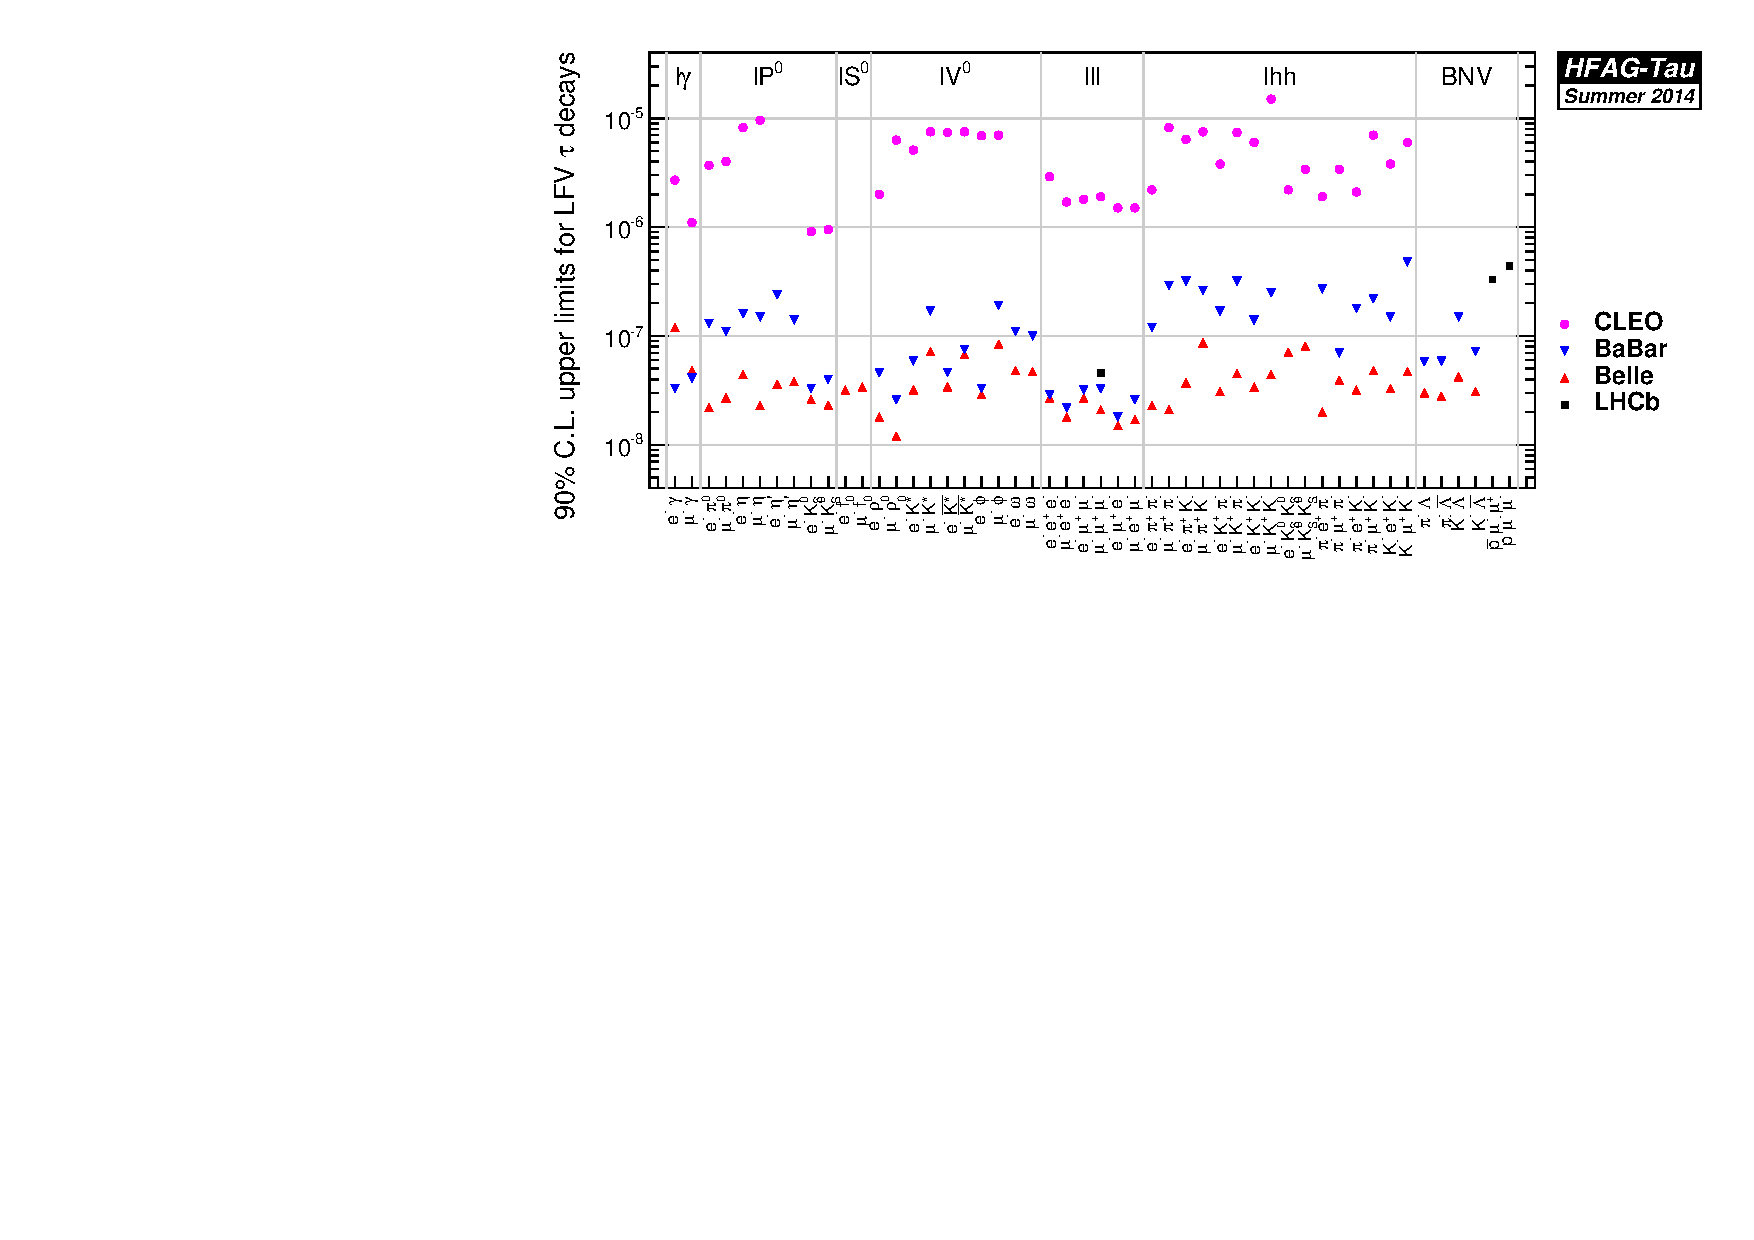
\includegraphics[angle=270,totalheight=0.9\textheight,clip]{TauLFV_limits.pdf}
    \caption{Tau lepton-flavor-violating branching fraction upper
      limits summary plot.
      \label{fig:tau:lfv-limits-plot}
    }
  \end{center}
\end{figure}
